\documentclass[11pt,a4paper]{article}

% ── Packages ──────────────────────────────────────────────────────────
\usepackage[utf8]{inputenc}
\usepackage[T1]{fontenc}
\usepackage{lmodern}
\usepackage[margin=2.5cm]{geometry}
\usepackage{booktabs}
\usepackage{tabularx}
\usepackage{array}
\usepackage{xcolor}
\usepackage{hyperref}
\usepackage{fancyhdr}
\usepackage{enumitem}
\usepackage{amssymb}
\usepackage{amsmath}
\usepackage{graphicx}
\usepackage{float}
\usepackage{tcolorbox}
\usepackage{tikz}

% ── Colours ───────────────────────────────────────────────────────────
\definecolor{ee8blue}{RGB}{0,90,160}
\definecolor{ee8gray}{RGB}{100,100,100}
\definecolor{warnbg}{RGB}{255,250,230}
\definecolor{warnborder}{RGB}{220,180,50}
\definecolor{notebg}{RGB}{235,245,255}
\definecolor{noteborder}{RGB}{70,130,200}
\definecolor{hintbg}{RGB}{235,255,235}
\definecolor{hintborder}{RGB}{60,160,60}

% ── tcolorbox styles ─────────────────────────────────────────────────
\newtcolorbox{designnote}{
  colback=notebg, colframe=noteborder,
  fonttitle=\bfseries, title=Design Note,
  boxrule=0.5pt, arc=2pt,
  left=6pt, right=6pt, top=4pt, bottom=4pt,
}
\newtcolorbox{warningbox}{
  colback=warnbg, colframe=warnborder,
  fonttitle=\bfseries, title=Important,
  boxrule=0.5pt, arc=2pt,
  left=6pt, right=6pt, top=4pt, bottom=4pt,
}
\newtcolorbox{hintbox}{
  colback=hintbg, colframe=hintborder,
  fonttitle=\bfseries, title=Hint,
  boxrule=0.5pt, arc=2pt,
  left=6pt, right=6pt, top=4pt, bottom=4pt,
}

% ── Hyperref setup ────────────────────────────────────────────────────
\hypersetup{
  colorlinks=true,
  linkcolor=ee8blue,
  urlcolor=ee8blue,
  pdftitle={EG2300 Tutorial 15 -- Program Counter with T Flip-Flops},
  pdfauthor={EG2300 Course Team},
}

% ── Header / footer ──────────────────────────────────────────────────
\pagestyle{fancy}
\fancyhf{}
\fancyhead[L]{\small\textcolor{ee8gray}{EG2300 --- Tutorial 15}}
\fancyhead[R]{\small\textcolor{ee8gray}{Program Counter (T~Flip-Flops)}}
\fancyfoot[C]{\small\textcolor{ee8gray}{\thepage}}
\renewcommand{\headrulewidth}{0.4pt}
\renewcommand{\footrulewidth}{0pt}

% ── Convenience ──────────────────────────────────────────────────────
\newcommand{\signal}[1]{\texttt{#1}}

\begin{document}

% ── Title ────────────────────────────────────────────────────────────
\begin{center}
  {\LARGE\bfseries EG2300 --- Engineering Design II}\\[6pt]
  {\Large Program Counter with T~Flip-Flops}\\[4pt]
  {\large Adding Unconditional Jump}
\end{center}
\vspace{1em}

% ═════════════════════════════════════════════════════════════════════
\section{Context}
% ═════════════════════════════════════════════════════════════════════

In Tutorial~14 you built a Program Counter using T~flip-flops that can
count up and reset to zero.
In this workshop you will add \textbf{unconditional jump} functionality
--- the ability to load an arbitrary 4-bit address into the PC using the
asynchronous set/clear pins.
You will also need to ensure that your existing reset still works correctly
\emph{alongside} the new jump logic.

% ═════════════════════════════════════════════════════════════════════
\section{Learning Objectives}
% ═════════════════════════════════════════════════════════════════════

By the end of this workshop you should be able to:
\begin{enumerate}[leftmargin=2em]
  \item Use the \textbf{asynchronous set/clear} pins on T~flip-flops to load an arbitrary value (jump).
  \item Modify existing reset logic so that reset and jump \textbf{coexist safely} (no Set/Clear conflicts).
  \item Verify that \textbf{priority} is correct: reset overrides jump, jump overrides counting.
\end{enumerate}

% ═════════════════════════════════════════════════════════════════════
\section{T~Flip-Flop Recap}
% ═════════════════════════════════════════════════════════════════════

A T~(toggle) flip-flop has the following behaviour:

\begin{center}
\begin{tabular}{ccl}
  \toprule
  \textbf{T} & \textbf{Clock edge} & \textbf{Q (next)} \\
  \midrule
  0 & $\uparrow$ & $Q$ \quad (hold) \\
  1 & $\uparrow$ & $\overline{Q}$ \quad (toggle) \\
  \bottomrule
\end{tabular}
\end{center}

\medskip
In Logisim the T~flip-flop also has two \textbf{asynchronous} pins on the bottom:

\begin{center}
\begin{tabular}{cll}
  \toprule
  \textbf{Pin label} & \textbf{Name} & \textbf{Effect (active = 1)} \\
  \midrule
  \texttt{1} & Preset (Set) & Forces $Q = 1$ immediately, ignores clock \\
  \texttt{0} & Clear (Reset) & Forces $Q = 0$ immediately, ignores clock \\
  \bottomrule
\end{tabular}
\end{center}

\begin{warningbox}
If both the Set and Clear pins are driven high at the same time,
Clear wins and $Q$ is forced to \textbf{0}.
While not an error in Logisim, this is \textbf{ambiguous behaviour} on real
hardware --- your logic should guarantee it never happens.
\end{warningbox}

\paragraph{Experiment: See it for yourself.}
Before building the full counter, place a \emph{single} T~flip-flop and
explore its three bottom pins.

\begin{figure}[H]
  \centering
  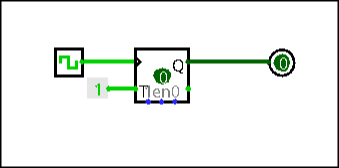
\includegraphics[width=0.35\textwidth]{img/FF-Off.jpg}\hfill
  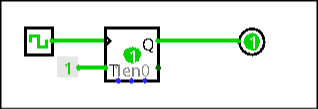
\includegraphics[width=0.35\textwidth]{img/FF-On.jpg}
  \caption{T~=~1 causes Q to toggle on every rising clock edge (Q\,=\,0 $\to$ Q\,=\,1).}
\end{figure}

\begin{figure}[H]
  \centering
  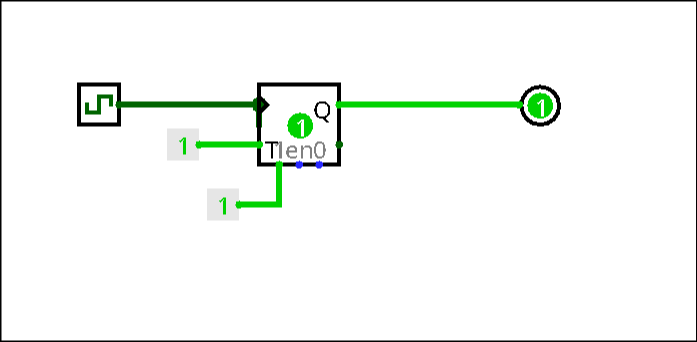
\includegraphics[width=0.55\textwidth]{img/AsyncSetHI.jpg}
  \caption{Async Set (pin ``1'') forces $Q = 1$ without a clock edge.}
\end{figure}

\begin{figure}[H]
  \centering
  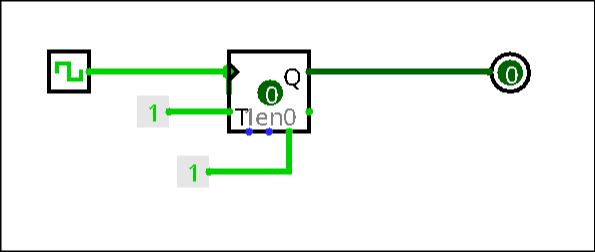
\includegraphics[width=0.55\textwidth]{img/AsyncSetLO.jpg}
  \caption{Async Clear (pin ``0'') forces $Q = 0$. Normal counting resumes when released.}
\end{figure}

\begin{figure}[H]
  \centering
  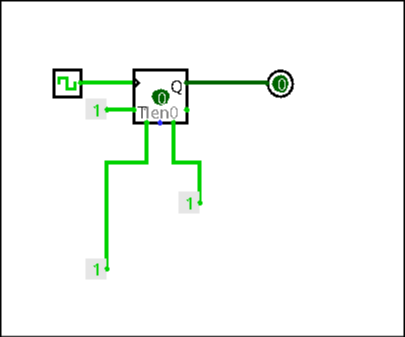
\includegraphics[width=0.45\textwidth]{img/AsyncSetHILO.jpg}
  \caption{Both Set and Clear active --- Clear wins in Logisim ($Q = 0$), but undefined on real hardware.}
\end{figure}

% ═════════════════════════════════════════════════════════════════════
\section{Required Behaviour}
% ═════════════════════════════════════════════════════════════════════

The Program Counter is a 4-bit value stored across four T~flip-flops.
Three operations are possible, with the following \textbf{strict priority}:

\begin{center}
\renewcommand{\arraystretch}{1.3}
\begin{tabular}{clll}
  \toprule
  \textbf{Priority} & \textbf{Condition} & \textbf{Action} & \textbf{Mechanism} \\
  \midrule
  1 (highest) & \signal{RST} = 1      & PC $\leftarrow$ 0000   & Async clear all FFs \\
  2           & \signal{JMP\_EN} = 1   & PC $\leftarrow$ \signal{ADDR} & Async set/clear per bit \\
  3 (default) & Neither                & PC $\leftarrow$ PC + 1 & T-input toggle chain \\
  \bottomrule
\end{tabular}
\end{center}

% ═════════════════════════════════════════════════════════════════════
\section{Interface Specification}
% ═════════════════════════════════════════════════════════════════════

Create a subcircuit called \signal{ProgramCounter\_TFF} with the following pins.

\begin{center}
\renewcommand{\arraystretch}{1.2}
\begin{tabular}{llcl}
  \toprule
  \textbf{Name} & \textbf{Width} & \textbf{Dir.} & \textbf{Meaning} \\
  \midrule
  \signal{CLK}       & 1 & in  & System clock (rising-edge) \\
  \signal{RST}       & 1 & in  & Asynchronous reset (PC $\leftarrow$ 0) \\
  \signal{JMP\_EN}   & 1 & in  & Jump enable \\
  \signal{ADDR[3:0]} & 4 & in  & Jump target address \\
  \signal{PC\_OUT[3:0]} & 4 & out & Current program counter value \\
  \bottomrule
\end{tabular}
\end{center}

% ═════════════════════════════════════════════════════════════════════
\section{Tasks}
% ═════════════════════════════════════════════════════════════════════

% ─────────────────────────────────────────────────────────────────────
\subsection{Part A --- Starting Point}
% ─────────────────────────────────────────────────────────────────────

\textbf{Goal:} Verify your existing Program Counter from Tutorial~14 before
modifying it.

You should already have:
\begin{itemize}[leftmargin=2em]
  \item Four T~flip-flops wired as a ripple-carry counter (counting 0--15).
  \item A \signal{RST} input that clears all flip-flops to 0 (via the async
        Clear pins).
\end{itemize}

\paragraph{Test A.}
\begin{itemize}
  \item Toggle \signal{CLK} manually --- confirm output counts
        $0000 \to 0001 \to \ldots \to 1111 \to 0000$.
  \item Assert \signal{RST} --- confirm output resets to $0000$.
  \item If either is broken, fix it before proceeding.
\end{itemize}


% ─────────────────────────────────────────────────────────────────────
\subsection{Part B --- Add Unconditional Jump}
% ─────────────────────────────────────────────────────────────────────

\textbf{Goal:} When \signal{JMP\_EN} is asserted, force the PC to the value
on \signal{ADDR[3:0]} using the async set/clear pins.

Currently your Clear pins are driven by \signal{RST} alone.
You will now use \emph{both} the Set and Clear pins on each flip-flop
to write an arbitrary address --- while keeping reset working.

\paragraph{The problem.}
Your existing reset wires \signal{RST} directly to every Clear pin.
If you also wire jump logic to the Clear pins, you need to make sure:
\begin{enumerate}[leftmargin=2em]
  \item Jump can drive both Set \emph{and} Clear (to write 1s and 0s).
  \item Reset still overrides jump (if both are active, reset wins).
  \item Set and Clear are \textbf{never both high} on the same flip-flop.
\end{enumerate}

\paragraph{Per-bit equations.} For each bit $i \in \{0,1,2,3\}$:

\begin{align}
  \text{SET}_i  &= \overline{\signal{RST}} \;\texttt{AND}\;
                    \signal{JMP\_EN} \;\texttt{AND}\; \signal{ADDR}[i]
    \label{eq:set} \\[4pt]
  \text{CLR}_i  &= \signal{RST} \;\texttt{OR}\;
                    \bigl(\signal{JMP\_EN} \;\texttt{AND}\;
                    \overline{\signal{ADDR}[i]}\bigr)
    \label{eq:clr}
\end{align}

\begin{itemize}[leftmargin=2em]
  \item If \signal{ADDR}$[i] = 1$ and \signal{RST}$= 0$:
        Set fires $\Rightarrow Q_i = 1$.
  \item If \signal{ADDR}$[i] = 0$:
        Clear fires $\Rightarrow Q_i = 0$.
  \item If \signal{RST}$= 1$: Set is forced to 0, Clear is forced to 1
        $\Rightarrow Q_i = 0$ regardless of jump. \textbf{Reset wins.}
  \item If \signal{JMP\_EN}$= 0$ and \signal{RST}$= 0$:
        both pins are 0 $\Rightarrow$ normal clocked counting.
\end{itemize}

\begin{designnote}
Verify for yourself that SET$_i$ and CLR$_i$ can never both be 1:
\begin{itemize}[nosep]
  \item \signal{RST}~=~1 $\Rightarrow$ SET$_i = 0$ (because of $\overline{\text{RST}}$),
        CLR$_i = 1$. \checkmark
  \item \signal{JMP\_EN}~=~1, \signal{RST}~=~0, \signal{ADDR}$[i]=1$
        $\Rightarrow$ SET$_i = 1$, CLR$_i = 0$. \checkmark
  \item \signal{JMP\_EN}~=~1, \signal{RST}~=~0, \signal{ADDR}$[i]=0$
        $\Rightarrow$ SET$_i = 0$, CLR$_i = 1$. \checkmark
  \item \signal{JMP\_EN}~=~0, \signal{RST}~=~0
        $\Rightarrow$ SET$_i = 0$, CLR$_i = 0$. \checkmark
\end{itemize}
No conflict in any case.
\end{designnote}

\paragraph{Disable counting during jump.}
When \signal{JMP\_EN} is active, the T-inputs must be forced to 0 so the
clock edge does not also toggle the flip-flops.
Replace the constant~1 feeding $T_0$:

\[
  T_0 = \overline{\signal{JMP\_EN}}
\]

The carry chain naturally propagates the zero, since
$T_1 = \overline{\signal{JMP\_EN}} \;\texttt{AND}\; Q_0$, etc.

\begin{designnote}
Why disable T during a jump? The async pins override Q \emph{instantly}, but
the next clock edge would also toggle Q if $T = 1$.
Without the NOT gate on $T_0$, a jump to address $A$ could immediately
become $A+1$ on the same clock edge --- defeating the purpose of the jump.
\end{designnote}

\paragraph{Build instructions.}
\begin{enumerate}[leftmargin=2em]
  \item Add a 4-bit \signal{ADDR} input pin and a splitter to break it into
        individual bits.
  \item Add a \signal{JMP\_EN} input pin.
  \item Add shared NOT gates: $\overline{\signal{RST}}$ and
        $\overline{\signal{JMP\_EN}}$.
  \item For each bit $i$, place:
    \begin{itemize}
      \item One NOT gate (inverts \signal{ADDR}$[i]$).
      \item One 3-input AND gate for SET$_i$
            (Equation~\ref{eq:set}: $\overline{\text{RST}}$, JMP\_EN, ADDR$[i]$).
      \item One 2-input AND gate for the inner term
            (JMP\_EN $\texttt{AND}$ $\overline{\text{ADDR}[i]}$).
      \item One 2-input OR gate for CLR$_i$
            (Equation~\ref{eq:clr}: RST $\texttt{OR}$ inner).
    \end{itemize}
  \item Wire SET$_i$ to the flip-flop's \texttt{``1''} pin.
  \item \textbf{Replace} the existing direct RST $\to$ Clear wire with
        CLR$_i$ from the OR gate.
  \item Replace the constant~1 on $T_0$ with $\overline{\signal{JMP\_EN}}$.
\end{enumerate}

\paragraph{Test B.}
\begin{itemize}
  \item Let the counter run to some value (e.g.\ 0011).
  \item Set \signal{ADDR} $= 1010$ and pulse \signal{JMP\_EN}.
  \item Verify \signal{PC\_OUT} immediately shows $1010$.
  \item Release \signal{JMP\_EN} and clock again --- counter resumes from $1011$.
\end{itemize}

\begin{figure}[H]
  \centering
  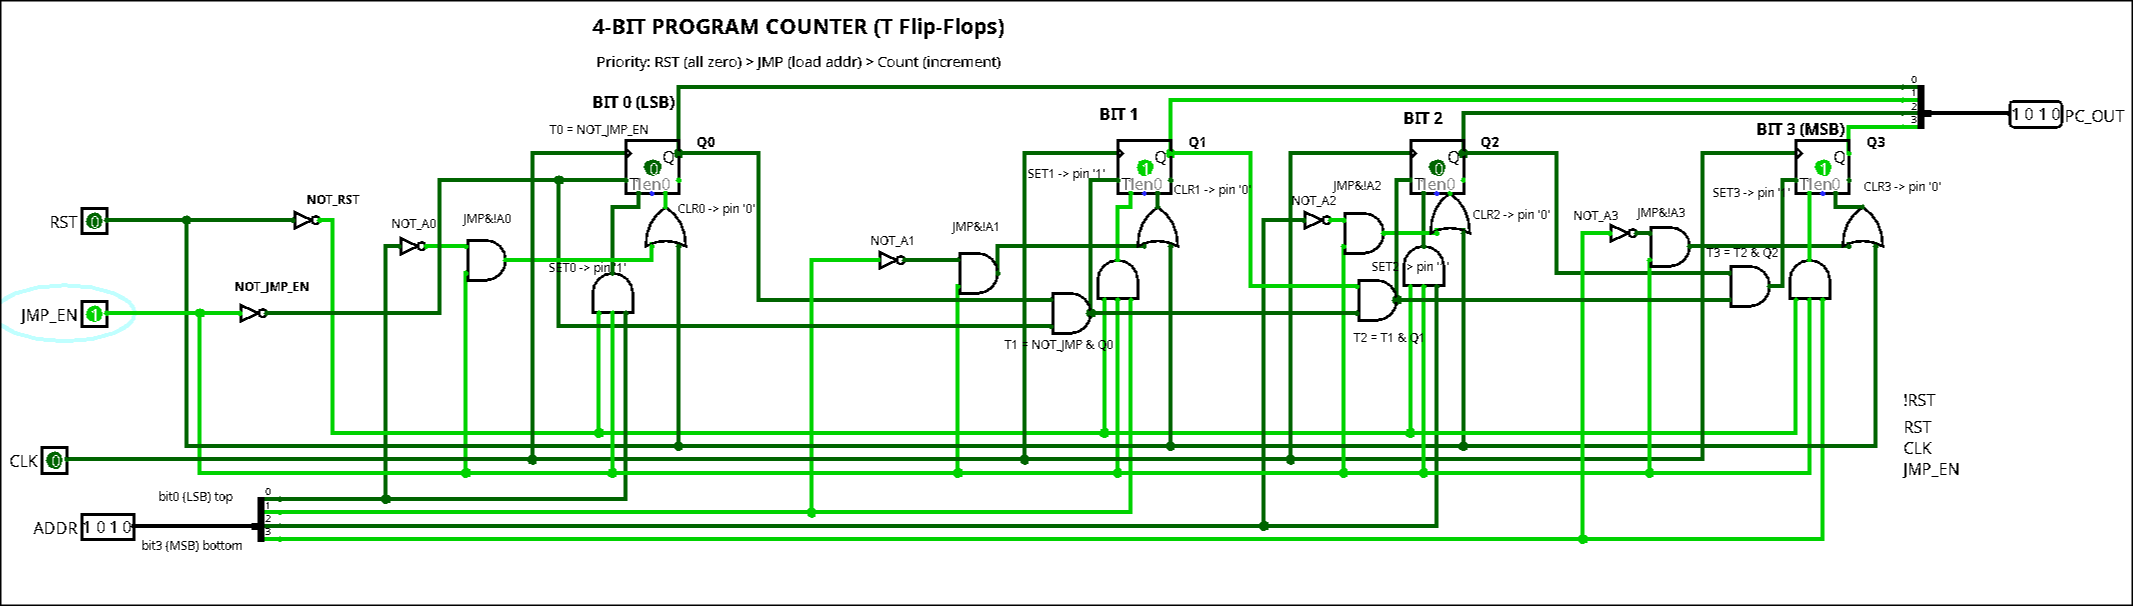
\includegraphics[width=\textwidth]{img/JMPEnable.jpg}
  \caption{Jump active --- \signal{ADDR}\,=\,1010, \signal{JMP\_EN}\,=\,1. PC\_OUT shows 1010; T-inputs are forced to 0.}
\end{figure}

\begin{figure}[H]
  \centering
  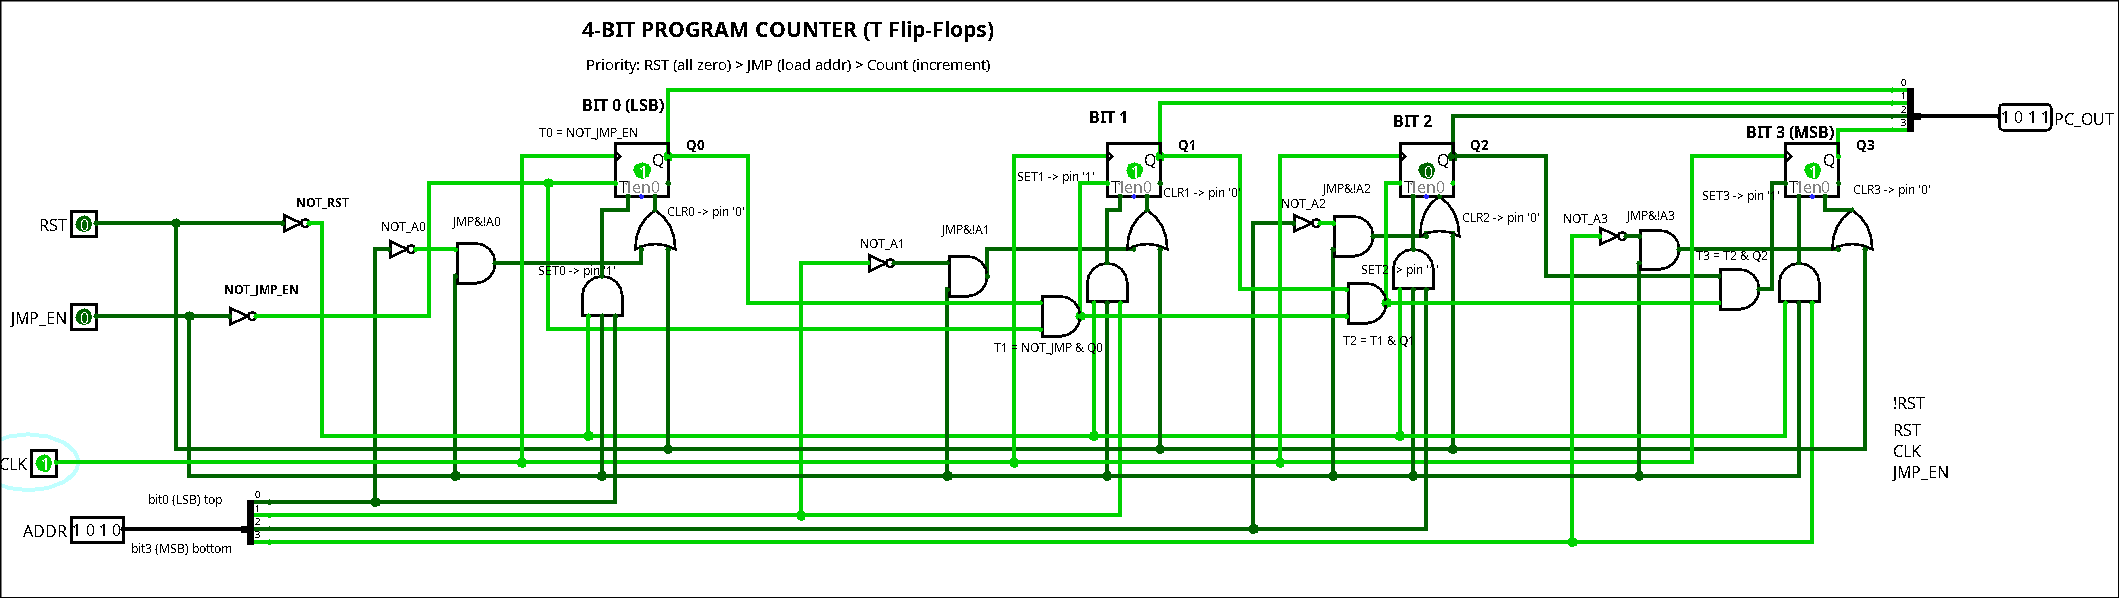
\includegraphics[width=\textwidth]{img/JMP_NotEN_Tick.jpg}
  \caption{After releasing \signal{JMP\_EN} and clocking once, the counter resumes from the loaded value.}
\end{figure}

% ─────────────────────────────────────────────────────────────────────
\subsection{Part C --- Verify Priority}
% ─────────────────────────────────────────────────────────────────────

\textbf{Goal:} Confirm that reset, jump, and counting interact correctly.

\paragraph{Test C --- reset overrides jump.}
\begin{itemize}
  \item Run counter to 0110.
  \item Assert \signal{RST}. Verify \signal{PC\_OUT} = 0000 immediately.
  \item While \signal{RST} is held, also assert \signal{JMP\_EN} with
        \signal{ADDR}~=~1111. Verify \signal{PC\_OUT} \textbf{stays 0000}
        (reset wins).
  \item Release \signal{RST} (keep \signal{JMP\_EN} high).
        Verify \signal{PC\_OUT} jumps to 1111.
  \item Release \signal{JMP\_EN}, clock once. Verify counter resumes: 0000.
\end{itemize}

\begin{figure}[H]
  \centering
  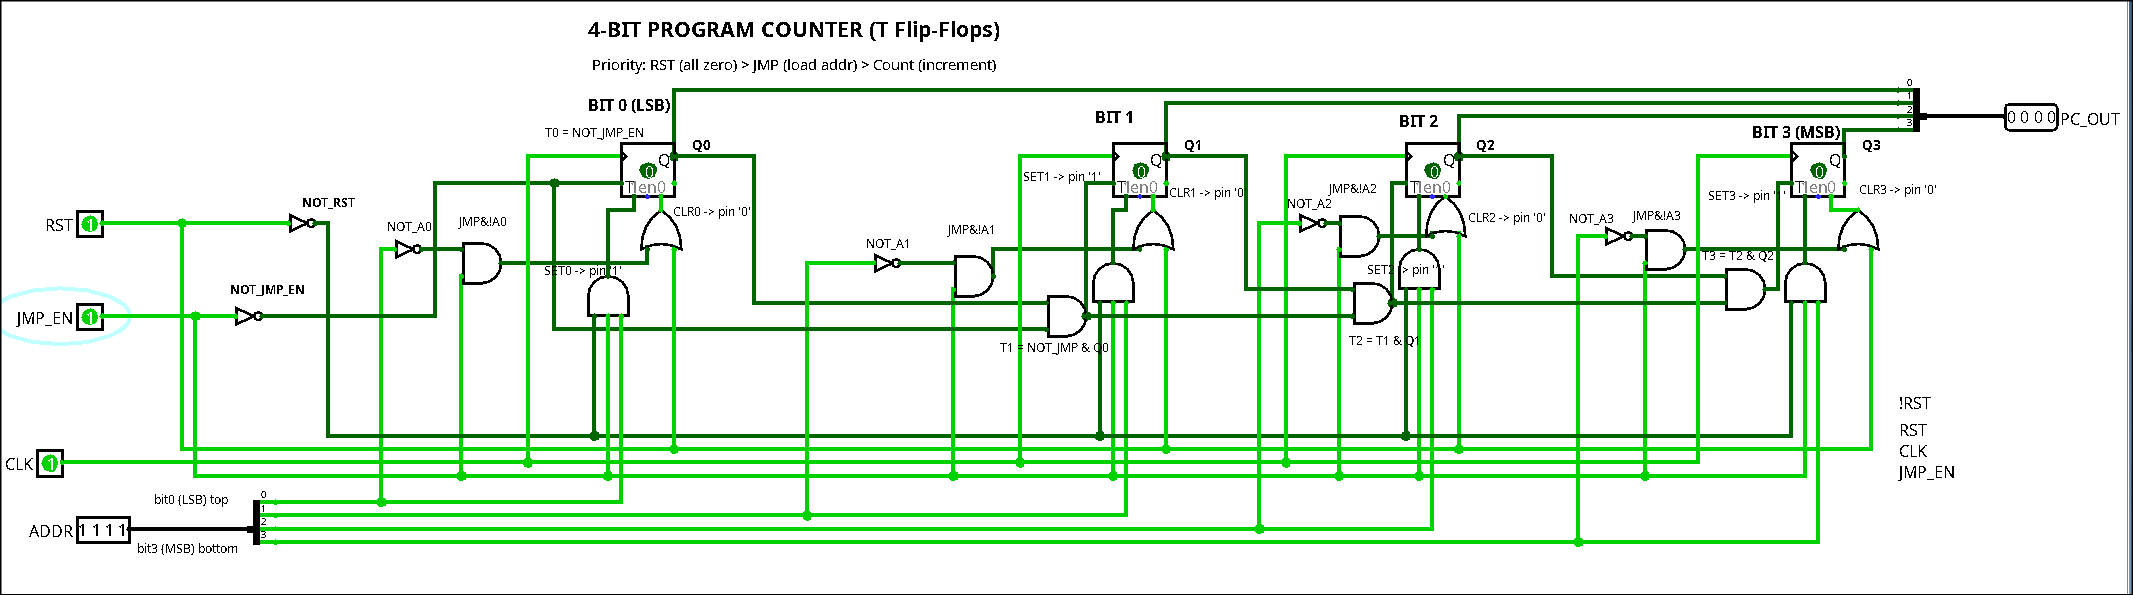
\includegraphics[width=\textwidth]{img/RST_OVERRIDE.jpg}
  \caption{Reset overrides jump --- \signal{RST}\,=\,1 and \signal{JMP\_EN}\,=\,1 with \signal{ADDR}\,=\,1111, yet PC\_OUT stays 0000.}
\end{figure}

% ═════════════════════════════════════════════════════════════════════
\section{Summary of Equations}
% ═════════════════════════════════════════════════════════════════════

For reference, the complete logic for each flip-flop bit $i$:

\begin{center}
\renewcommand{\arraystretch}{1.4}
\begin{tabular}{ll}
  \toprule
  \textbf{Signal} & \textbf{Equation} \\
  \midrule
  $\text{SET}_i$ & $\overline{\text{RST}} \;\texttt{AND}\; \text{JMP\_EN}
                     \;\texttt{AND}\; \text{ADDR}[i]$ \\
  $\text{CLR}_i$ & $\text{RST} \;\texttt{OR}\; (\text{JMP\_EN}
                     \;\texttt{AND}\; \overline{\text{ADDR}[i]})$ \\
  $T_0$          & $\overline{\text{JMP\_EN}}$ \\
  $T_1$          & $\overline{\text{JMP\_EN}} \;\texttt{AND}\; Q_0$ \\
  $T_2$          & $T_1 \;\texttt{AND}\; Q_1$ \quad (carry chain) \\
  $T_3$          & $T_2 \;\texttt{AND}\; Q_2$ \quad (carry chain) \\
  \bottomrule
\end{tabular}
\end{center}

% ═════════════════════════════════════════════════════════════════════
\section{What to Save}
% ═════════════════════════════════════════════════════════════════════

Your file must include the following subcircuit:
\begin{itemize}
  \item \signal{ProgramCounter\_TFF}
\end{itemize}

% ═════════════════════════════════════════════════════════════════════
\section{Optional Extension}
% ═════════════════════════════════════════════════════════════════════

If you finish early:
\begin{enumerate}[leftmargin=2em]
  \item \textbf{ROM integration.} Connect \signal{PC\_OUT} to your instruction
        ROM from Tutorial~13 and verify the PC steps through stored instructions
        automatically.
  \item \textbf{Conditional branch.} Add external combinational logic that
        checks a register value and drives \signal{JMP\_EN} only when the
        condition is met (e.g.\ jump-if-zero/jump-if-not-zero [JZ/JNZ]).
  \item \textbf{HALT.} Add a \signal{HALT} input that freezes the PC
        (forces all T-inputs to 0 and disables set/clear).
\end{enumerate}

\end{document}
